\documentclass[conference]{IEEEtran}

% ============================================================
% Packages
% ============================================================
\usepackage{amsmath,amssymb,amsfonts}
\usepackage{algorithm}
\usepackage{algorithmic}
\usepackage{booktabs}
\usepackage{multirow}
\usepackage{graphicx}
\usepackage{xcolor}
\usepackage{url}
\usepackage{tikz}
\usepackage{pgfplots}
\usepackage{balance}

\usetikzlibrary{
    arrows.meta,
    positioning,
    shapes.geometric,
    fit,
    calc,
    backgrounds
}

\pgfplotsset{compat=1.18}

% ============================================================
% Custom commands
% ============================================================
\newcommand{\method}{LearnedPPR}
\newcommand{\ppr}{PPR}
\newcommand{\q}{q}
\newcommand{\graph}{G}
\newcommand{\reset}{r}
\newcommand{\gatedreset}{\tilde r}
\newcommand{\policy}{\pi_{\theta}}

% ============================================================
% Title
% ============================================================
\title{
Query-Adaptive Personalization Policy for\\
Multi-Granular Graph Retrieval
}

% ============================================================
% Authors
% ============================================================
\author{
\IEEEauthorblockN{Anonymous Authors}
\IEEEauthorblockA{
Anonymous Institution\\
Anonymous City, Country\\
email@anonymous.org
}
}

\begin{document}

\maketitle

% ============================================================
% Abstract
% ============================================================
\begin{abstract}
Graph-based retrieval methods exploit relational structures among
passages, entities, and documents to improve multi-hop evidence
retrieval. However, existing approaches typically employ a fixed
personalization strategy for different queries, although queries may
require substantially different retrieval behaviors. A query may, for
example, benefit from entity-level evidence, passage-level evidence,
or document-level context, and may require either local evidence
aggregation or broader graph diffusion.

We propose \method, a query-adaptive personalization framework for
multi-granular graph retrieval. Instead of directly learning a new
graph structure or modifying the transition matrix of Personalized
PageRank (PPR), \method learns a shared query-conditioned policy that
generates a compact set of control variables for each query. These
variables determine (i) the relative importance of different node
granularities, (ii) the selectivity of semantic node gating, and
(iii) the persistence of graph diffusion. The resulting query-aware
node gates reweight the PPR personalization vector before graph
propagation, while a query-dependent damping factor controls the
balance between personalization and graph structure.

This formulation preserves the original graph and PPR propagation
mechanism while allowing the retrieval behavior to adapt to each
query. Experiments on graph-based retrieval demonstrate that the
proposed method substantially improves retrieval recall over the
underlying PPR-based baseline, achieving a Recall@5 of 89.05\% and
Recall@10 of 93.80\%. Further ablations investigate the contributions
of granularity routing, semantic selectivity, and adaptive diffusion.
\end{abstract}

\begin{IEEEkeywords}
graph retrieval, personalized PageRank, query-adaptive retrieval,
knowledge graph, multi-granular retrieval, neural policy
\end{IEEEkeywords}

% ============================================================
% 1. Introduction
% ============================================================
\section{Introduction}

Retrieving relevant evidence from a large collection of documents is
a fundamental problem in modern question answering and information
retrieval. Dense retrieval methods provide effective semantic
matching between queries and passages, but they may struggle when
relevant evidence is distributed across multiple documents or linked
through entities and higher-level semantic relations. Graph-based
retrieval addresses this limitation by representing documents,
passages, and entities as nodes and exploiting graph connectivity to
propagate relevance across related evidence.

Personalized PageRank (PPR) is particularly attractive for graph
retrieval because it combines query-derived personalization with
graph-based diffusion. Given a graph $G=(V,E)$ and a personalization
vector $\reset$, PPR computes a stationary relevance distribution
according to
\begin{equation}
\mathbf{p}
=
d\reset
+
(1-d)\mathbf{P}^{\top}\mathbf{p},
\label{eq:ppr}
\end{equation}
where $\mathbf{P}$ is the graph transition matrix and $d$ is the
teleportation or reset probability. The personalization vector
determines where probability mass is injected into the graph, while
the transition matrix determines how this mass propagates.

Despite its effectiveness, a key limitation of conventional
graph-based retrieval is that the same propagation behavior is often
used for all queries. This assumption is restrictive because queries
can differ substantially in their information needs. Some queries are
primarily entity-oriented, while others require passage-level
evidence or document-level context. Similarly, some queries are
well-served by highly selective local evidence, whereas others benefit
from broader graph diffusion.

This observation motivates the following question:

\begin{quote}
\emph{Can the personalization and diffusion behavior of graph
retrieval be dynamically adapted to the semantic characteristics of
each query?}
\end{quote}

We address this question with \method, a query-adaptive
personalization policy for multi-granular graph retrieval. The key
idea is to retain the original graph and PPR propagation mechanism,
while learning how the personalization distribution should be adapted
for each query. Specifically, a shared policy network
$\policy(\q)$ predicts query-specific control variables that determine
three aspects of retrieval behavior: granularity allocation,
semantic selectivity, and diffusion persistence.

For each graph node $v$, the policy produces a query-dependent gate
\begin{equation}
g_v(\q)
=
w_{T(v),\q}
\sigma
\left(
k_{T(v),\q}
\left[
s(\q,v)-\tau_{T(v),\q}
\right]
\right),
\label{eq:gate}
\end{equation}
where $T(v)$ denotes the node type, $s(\q,v)$ is the semantic
similarity between the query and node $v$, $w_{T(v),\q}$ is a
query-dependent granularity weight, $\tau_{T(v),\q}$ is a
query-dependent selectivity threshold, and $k_{T(v),\q}$ controls the
sharpness of the gate.

The gate is applied to the entire graph-level personalization vector:
\begin{equation}
\gatedreset_v
=
\reset_v g_v(\q).
\label{eq:gated-reset}
\end{equation}
After normalization, this query-adaptive personalization vector is
used as the reset distribution of PPR. Importantly, \method does not
modify the graph transition matrix. Therefore, the method can be
viewed as learning \emph{where the diffusion should start} and
\emph{how strongly it should persist}, rather than learning a new
graph topology.

Our contributions are summarized as follows:

\begin{itemize}
    \item We formulate graph retrieval as a
    \emph{query-adaptive personalization} problem, where a shared
    policy dynamically generates a query-specific personalization
    strategy rather than using a fixed PPR reset distribution.

    \item We introduce a multi-granular node gating mechanism that
    jointly models granularity allocation and query-dependent
    semantic selectivity across entity, passage, and paper nodes.

    \item We introduce query-dependent diffusion control through an
    adaptive PPR damping factor, allowing different queries to favor
    either personalization-driven retrieval or broader graph
    diffusion.

    \item Experiments demonstrate substantial improvements over the
    underlying PPR-based retrieval system, while ablation studies
    analyze the individual contributions of adaptive gating,
    granularity routing, and diffusion control.
\end{itemize}


% ============================================================
% 2. Related Work
% ============================================================
\section{Related Work}

\subsection{Dense and Graph-Based Retrieval}

Dense retrieval represents queries and documents in a continuous
embedding space and retrieves candidates according to semantic
similarity. Although effective for direct semantic matching, dense
retrieval may have difficulty recovering evidence that is not directly
similar to the query but is connected through intermediate entities or
documents.

Graph-based retrieval augments semantic retrieval with relational
information. A graph can connect passages, documents, and entities,
allowing relevance to propagate across multiple hops. This property
is especially useful for multi-hop retrieval, where the final relevant
passage may have weak lexical or semantic similarity to the original
query but strong structural connections to intermediate evidence.

\subsection{Personalized PageRank for Retrieval}

Personalized PageRank provides a principled mechanism for combining
query-dependent initialization with graph diffusion. Given a
personalization vector $\reset$, PPR repeatedly propagates probability
mass through the graph while periodically returning probability mass
to the personalized nodes.

Existing graph retrieval systems typically construct $\reset$ from
retrieval results or query-related evidence and then apply a fixed
PPR procedure. In contrast, \method learns how this personalization
should be adapted to the query.

\subsection{Adaptive Retrieval Policies}

Neural policies have been explored for adaptive retrieval, including
adaptive query expansion, document selection, and retrieval strategy
selection. Our approach differs in that the policy does not directly
select a final passage list. Instead, it controls the intermediate
probability distribution that drives graph diffusion. This provides a
compact interface between a neural query encoder and an otherwise
unchanged graph retrieval engine.


% ============================================================
% 3. Problem Formulation
% ============================================================
\section{Problem Formulation}

Let
\begin{equation}
G=(V,E)
\end{equation}
denote a heterogeneous graph containing entity, passage, and paper
nodes:
\begin{equation}
V=V_E\cup V_P\cup V_D.
\end{equation}

Given a query $\q$, an initial retrieval stage produces a set of
query-related evidence nodes. These nodes are converted into an
initial personalization vector
\begin{equation}
\reset\in\mathbb{R}^{|V|}.
\end{equation}

The baseline PPR retrieval process computes
\begin{equation}
\mathbf{p}
=
d\reset+(1-d)\mathbf{P}^{\top}\mathbf{p}.
\end{equation}

The final retrieval result consists of the top-$K$ passage nodes
according to $\mathbf{p}$.

The limitation of this formulation is that both the personalization
behavior and damping factor may be shared across queries. We instead
learn a query-conditioned policy
\begin{equation}
\Theta_{\q}
=
\policy(\operatorname{Embed}(\q)),
\label{eq:policy}
\end{equation}
which determines a query-specific personalization vector
$\reset_{\q}$ and damping factor $d_{\q}$:
\begin{equation}
\mathbf{p}_{\q}
=
d_{\q}\reset_{\q}
+
(1-d_{\q})\mathbf{P}^{\top}\mathbf{p}_{\q}.
\label{eq:adaptive-ppr}
\end{equation}

Thus, the graph transition matrix remains unchanged while the
query-specific retrieval behavior is introduced through the
personalization vector and diffusion persistence.


% ============================================================
% Figure 1: Overall architecture
% ============================================================
\begin{figure*}[t]
\centering

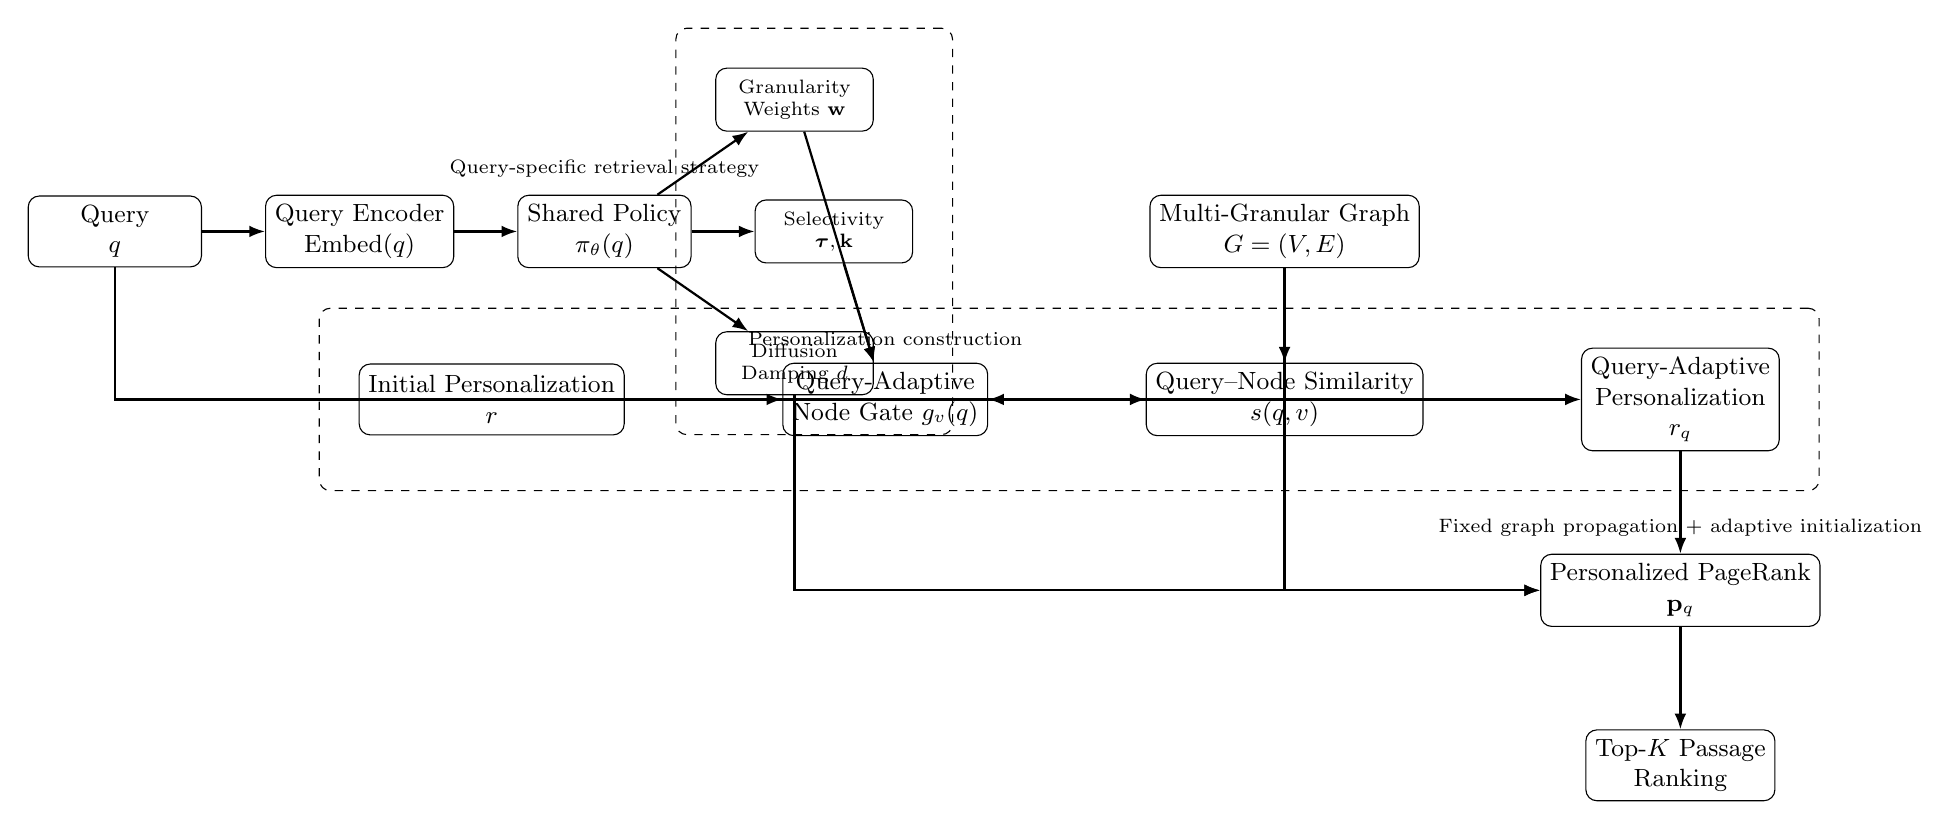
\begin{tikzpicture}[
    node distance=7mm and 8mm,
    box/.style={
        draw,
        rounded corners,
        minimum height=9mm,
        minimum width=22mm,
        align=center,
        font=\small
    },
    smallbox/.style={
        draw,
        rounded corners,
        minimum height=8mm,
        minimum width=20mm,
        align=center,
        font=\scriptsize
    },
    arrow/.style={
        -{Latex[length=2mm]},
        thick
    },
    group/.style={
        draw,
        dashed,
        rounded corners,
        inner sep=5mm
    }
]

\node[box] (query) {Query\\$\q$};
\node[box, right=of query] (encoder) {Query Encoder\\$\operatorname{Embed}(\q)$};
\node[box, right=of encoder] (policy) {Shared Policy\\$\policy(\q)$};

\node[smallbox, above right=8mm and 3mm of policy] (routing)
    {Granularity\\Weights $\mathbf{w}$};
\node[smallbox, right=of policy] (selectivity)
    {Selectivity\\$\boldsymbol{\tau},\mathbf{k}$};
\node[smallbox, below right=8mm and 3mm of policy] (damping)
    {Diffusion\\Damping $d$};

\node[box, right=30mm of selectivity] (graph)
    {Multi-Granular Graph\\$G=(V,E)$};

\node[box, below=12mm of graph] (sim)
    {Query--Node Similarity\\$s(\q,v)$};

\node[box, left=20mm of sim] (gate)
    {Query-Adaptive\\Node Gate $g_v(\q)$};

\node[box, left=20mm of gate] (reset)
    {Initial Personalization\\$\reset$};

\node[box, right=20mm of sim] (personal)
    {Query-Adaptive\\Personalization\\$\reset_{\q}$};

\node[box, below=13mm of personal] (ppr)
    {Personalized PageRank\\$\mathbf{p}_{\q}$};

\node[box, below=13mm of ppr] (result)
    {Top-$K$ Passage\\Ranking};

\draw[arrow] (query) -- (encoder);
\draw[arrow] (encoder) -- (policy);

\draw[arrow] (policy) -- (routing);
\draw[arrow] (policy) -- (selectivity);
\draw[arrow] (policy) -- (damping);

\draw[arrow] (routing) -- (gate);
\draw[arrow] (selectivity) -- (gate);

\draw[arrow] (reset) -- (gate);
\draw[arrow] (gate) -- (personal);

\draw[arrow] (query) |- (sim);
\draw[arrow] (graph) -- (sim);
\draw[arrow] (sim) -- (gate);

\draw[arrow] (personal) -- (ppr);
\draw[arrow] (damping) |- (ppr);
\draw[arrow] (graph) |- (ppr);

\draw[arrow] (ppr) -- (result);

\node[group, fit=(routing)(selectivity)(damping)] {};
\node[group, fit=(reset)(sim)(gate)(personal)] {};

\node[above=1mm of policy, font=\scriptsize]
    {Query-specific retrieval strategy};

\node[above=1mm of gate, font=\scriptsize]
    {Personalization construction};

\node[above=1mm of ppr, font=\scriptsize]
    {Fixed graph propagation + adaptive initialization};

\end{tikzpicture}

\caption{
Overview of \method. A shared query-conditioned policy predicts
granularity allocation, semantic selectivity, and diffusion
persistence. Query-dependent gates are computed for all nodes in the
multi-granular graph and are used to reweight the PPR personalization
vector. The graph transition matrix itself remains unchanged.
}
\label{fig:overview}
\end{figure*}


% ============================================================
% 4. Method
% ============================================================
\section{Query-Adaptive Personalization Policy}

\subsection{Shared Query-Conditioned Policy}

The central component of \method is a shared policy network:
\begin{equation}
\Theta_{\q}
=
\policy(\mathbf{q}),
\qquad
\mathbf{q}=\operatorname{Embed}(\q).
\end{equation}

The policy outputs ten scalar variables that are transformed into
three groups of granularity-specific parameters and one global
diffusion parameter.

The first three outputs are converted into granularity weights:
\begin{equation}
\mathbf{w}
=
(w_E,w_P,w_D)
=
\operatorname{softmax}(\Theta_{1:3}),
\label{eq:weights}
\end{equation}
where $E$, $P$, and $D$ denote entity, passage, and paper nodes,
respectively.

The next three outputs define semantic thresholds:
\begin{equation}
\tau_T
=
\sigma(\Theta_T),
\qquad
T\in\{E,P,D\}.
\label{eq:threshold}
\end{equation}

The following three outputs determine gate sharpness:
\begin{equation}
k_T
=
1+19\sigma(\Theta_T).
\label{eq:slope}
\end{equation}

Finally, the last output controls the PPR damping factor:
\begin{equation}
d_{\q}
=
0.3+0.65\sigma(\Theta_{10}).
\label{eq:damping}
\end{equation}

This parameterization constrains all policy outputs to meaningful
ranges and provides a compact representation of query-specific
retrieval behavior.


% ------------------------------------------------------------
% Figure 2: Gate
% ------------------------------------------------------------
\begin{figure}[t]
\centering

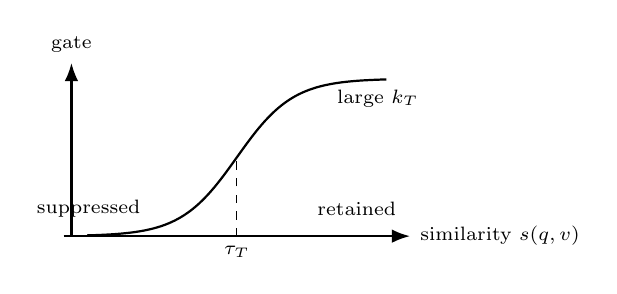
\begin{tikzpicture}[
    >=Latex,
    axis/.style={->, thick},
    gate/.style={thick}
]

\draw[axis] (-2.1,0) -- (2.3,0)
    node[right] {\scriptsize similarity $s(q,v)$};

\draw[axis] (-2.0,0) -- (-2.0,2.2)
    node[above] {\scriptsize gate};

\draw[gate]
    plot[smooth,domain=-1.8:2.0,samples=100]
    (\x,{2/(1+exp(-2.8*(\x-0.1)))});

\draw[dashed] (0.1,0) -- (0.1,1.0);

\node[below] at (0.1,0)
    {\scriptsize $\tau_T$};

\node[right] at (1.25,1.75)
    {\scriptsize large $k_T$};

\node[left] at (-1.0,0.35)
    {\scriptsize suppressed};

\node[right] at (1.0,0.35)
    {\scriptsize retained};

\end{tikzpicture}

\caption{
Illustration of the query-dependent sigmoid gate. The threshold
$\tau_T$ controls when a node starts receiving substantial
personalization mass, while $k_T$ controls the selectivity of the
transition.
}
\label{fig:gate}
\end{figure}


% ============================================================
% 4.2 Node Gating
% ============================================================
\subsection{Query-Adaptive Multi-Granular Node Gating}

For every node $v\in V$, we compute its semantic similarity to the
query:
\begin{equation}
s(\q,v)
=
\cos(\mathbf{q},\mathbf{e}_v),
\label{eq:similarity}
\end{equation}
where $\mathbf{e}_v$ is the embedding of node $v$.

The node type is denoted by $T(v)\in\{E,P,D\}$. The query-adaptive
gate is defined as:
\begin{equation}
g_v(\q)
=
w_{T(v)}
\sigma
\left(
k_{T(v)}
\left[
s(\q,v)-\tau_{T(v)}
\right]
\right).
\label{eq:nodegate}
\end{equation}

Unlike a fixed global filter, the policy produces different weights,
thresholds, and slopes for different queries. Consequently, the same
graph node can receive different gate values under different queries.

Importantly, gates are computed for all nodes in the graph rather than
only for initially retrieved nodes. This allows the policy to define a
query-conditioned relevance landscape over the heterogeneous graph.

The three components have distinct interpretations:

\begin{itemize}
    \item $w_T$ determines how much the policy favors a particular
    graph granularity;
    \item $\tau_T$ determines the semantic relevance required for a
    node to receive substantial gate value;
    \item $k_T$ determines whether the selection behavior is soft or
    sharply selective.
\end{itemize}


% ============================================================
% 4.3 Query Adaptive Personalization
% ============================================================
\subsection{Query-Adaptive Personalization}

Let $\reset$ denote the initial reset vector obtained from the
underlying fact retrieval and reranking procedure. We apply the
query-dependent gates element-wise:
\begin{equation}
\tilde r_v
=
r_v g_v(\q).
\label{eq:rawpersonalization}
\end{equation}

We then normalize the vector:
\begin{equation}
r_{\q,v}
=
\frac{\tilde r_v}
{\sum_{u\in V}\tilde r_u+\epsilon}.
\label{eq:normalization}
\end{equation}

The resulting vector $\reset_{\q}$ is the query-specific
personalization vector.

The interpretation of this operation is important. Each value
$r_{\q,v}$ represents the amount of probability mass assigned to node
$v$ when the PPR process resets. A larger value means that the node
acts as a stronger source of query-conditioned diffusion.

Thus, the policy does not directly rank the final passages. Instead,
it determines how much personalization mass should be allocated to
different nodes before graph propagation.


% ============================================================
% 4.4 Adaptive PPR
% ============================================================
\subsection{Adaptive Diffusion}

After constructing $\reset_{\q}$, we perform Personalized PageRank:
\begin{equation}
\mathbf{p}_{\q}
=
d_{\q}\reset_{\q}
+
(1-d_{\q})\mathbf{P}^{\top}\mathbf{p}_{\q}.
\label{eq:adaptiveppr}
\end{equation}

Equivalently,
\begin{equation}
\mathbf{p}_{\q}
=
d_{\q}
\sum_{t=0}^{\infty}
(1-d_{\q})^t
(\mathbf{P}^{\top})^t
\reset_{\q}.
\label{eq:series}
\end{equation}

Equation~\eqref{eq:series} provides a useful interpretation of
\method. The query-dependent gate determines the initial distribution
of diffusion mass, while $d_{\q}$ determines how quickly the influence
of this personalization distribution decays across graph hops.

The graph transition matrix $\mathbf{P}$ is not modified. Therefore,
\method preserves the structural inductive bias of the original graph
while adapting the query-dependent initialization and diffusion
persistence.


% ============================================================
% Figure 3: Personalization mass
% ============================================================
\begin{figure}[t]
\centering

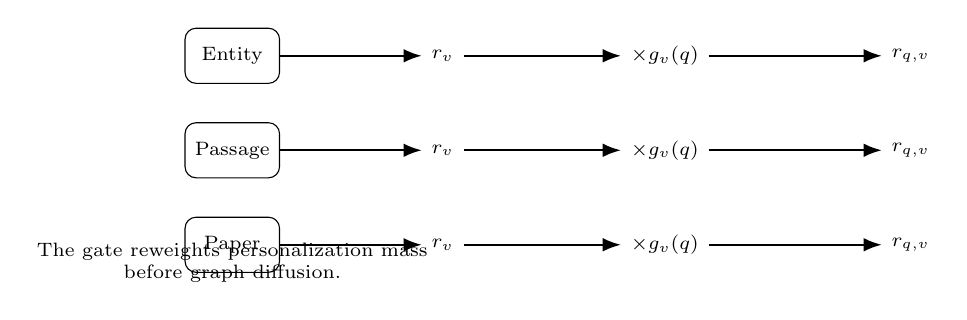
\begin{tikzpicture}[
    node/.style={
        draw,
        rounded corners,
        minimum width=12mm,
        minimum height=7mm,
        font=\scriptsize
    },
    arrow/.style={-{Latex},thick}
]

\node[node] (e1) at (0,1.8) {Entity};
\node[node] (p1) at (0,0.6) {Passage};
\node[node] (d1) at (0,-0.6) {Paper};

\node[right=18mm of e1, font=\scriptsize] (r1) {$r_v$};
\node[right=18mm of p1, font=\scriptsize] (r2) {$r_v$};
\node[right=18mm of d1, font=\scriptsize] (r3) {$r_v$};

\node[right=20mm of r1, font=\scriptsize] (g1) {$\times g_v(q)$};
\node[right=20mm of r2, font=\scriptsize] (g2) {$\times g_v(q)$};
\node[right=20mm of r3, font=\scriptsize] (g3) {$\times g_v(q)$};

\node[right=22mm of g1, font=\scriptsize] (o1) {$r_{q,v}$};
\node[right=22mm of g2, font=\scriptsize] (o2) {$r_{q,v}$};
\node[right=22mm of g3, font=\scriptsize] (o3) {$r_{q,v}$};

\draw[arrow] (e1) -- (r1);
\draw[arrow] (p1) -- (r2);
\draw[arrow] (d1) -- (r3);

\draw[arrow] (r1) -- (g1);
\draw[arrow] (r2) -- (g2);
\draw[arrow] (r3) -- (g3);

\draw[arrow] (g1) -- (o1);
\draw[arrow] (g2) -- (o2);
\draw[arrow] (g3) -- (o3);

\node[below=7mm of p1, font=\scriptsize, align=center]
{The gate reweights personalization mass\\
before graph diffusion.};

\end{tikzpicture}

\caption{
Query-adaptive personalization. The gate is computed for every node
and determines how much of the original personalization mass is
retained for each node.
}
\label{fig:personalization}
\end{figure}


% ============================================================
% 4.5 Complete Algorithm
% ============================================================
\subsection{Complete Retrieval Procedure}

The complete retrieval procedure is summarized in
Algorithm~\ref{alg:learnedppr}.

\begin{algorithm}[t]
\caption{Query-Adaptive \method Retrieval}
\label{alg:learnedppr}
\begin{algorithmic}[1]

\REQUIRE Query $\q$, graph $G=(V,E)$, trained policy $\policy$
\ENSURE Ranked passage list $R$

\STATE $\mathbf{q}\leftarrow\operatorname{Embed}(\q)$
\STATE $\Theta\leftarrow\policy(\mathbf{q})$

\STATE $\mathbf{w}\leftarrow\operatorname{softmax}(\Theta_{1:3})$
\STATE $\boldsymbol{\tau}\leftarrow\sigma(\Theta_{4:6})$
\STATE $\mathbf{k}\leftarrow1+19\sigma(\Theta_{7:9})$
\STATE $d\leftarrow0.3+0.65\sigma(\Theta_{10})$

\STATE $S\leftarrow\operatorname{FactRetrieval}(\q,G)$
\STATE $S\leftarrow\operatorname{Rerank}(\q,S)$
\STATE $\reset\leftarrow\operatorname{BuildResetVector}(S,|V|)$

\FOR{each node $v\in V$}
    \STATE $T\leftarrow\operatorname{NodeType}(v)$
    \STATE $s_v\leftarrow
    \cos(\mathbf{q},\mathbf{e}_v)$
    \STATE $g_v\leftarrow
    w_T\sigma(k_T(s_v-\tau_T))$
    \STATE $\tilde r_v\leftarrow r_vg_v$
\ENDFOR

\STATE $\reset_{\q}\leftarrow
\operatorname{Normalize}(\tilde{\reset})$

\STATE $\mathbf{p}_{\q}\leftarrow
\operatorname{PPR}(G,\reset_{\q},d)$

\STATE $R\leftarrow
\operatorname{TopK}
(\mathbf{p}_{\q}|_{V_P})$

\RETURN $R

\end{algorithmic}
\end{algorithm}


% ============================================================
% 5. Learning the Policy
% ============================================================
\section{Policy Learning}

\subsection{Training Objective}

The policy is trained from retrieval supervision. For each training
query $\q$, let $\mathcal{P}^{+}_{\q}$ denote the set of relevant
passages and $\mathcal{P}^{-}_{\q}$ denote negative passages.

The policy parameters $\theta$ are optimized to improve the final
graph retrieval ranking:
\begin{equation}
\theta^{*}
=
\arg\max_{\theta}
\mathcal{M}
\left(
R_{\q}(\theta),
\mathcal{P}^{+}_{\q}
\right),
\label{eq:objective}
\end{equation}
where $\mathcal{M}$ is the retrieval metric used during training or
policy optimization.

In implementation, the policy may be optimized using a pairwise
ranking objective, reinforcement learning, or another retrieval-aware
optimization procedure. In the current system, the policy is learned
jointly from retrieval supervision while the graph construction and
PPR inference procedure remain unchanged.

% TODO:
% Replace the above paragraph with the exact training algorithm
% actually used in the experiments.


% ============================================================
% 6. Experiments
% ============================================================
\section{Experiments}

\subsection{Experimental Setup}

\subsubsection{Dataset}

We evaluate \method on a graph-based paper retrieval benchmark
constructed from a corpus of research papers. Each paper is
represented using paper-, passage-, and entity-level nodes, with
edges encoding the corresponding semantic and document relations.

% TODO: Insert exact dataset size, number of queries,
% train/dev/test split, graph statistics, and source.

\subsubsection{Baselines}

We compare \method against the underlying PPR-based retrieval
framework and several increasingly adaptive variants.

\begin{itemize}
    \item \textbf{Base PPR}: the original graph retrieval system with
    a fixed personalization strategy.
    \item \textbf{Cosine Reweighting}: reweights the personalization
    vector using query-node semantic similarity without a learned
    policy.
    \item \textbf{Fixed Gate}: applies a shared sigmoid gate to all
    queries.
    \item \textbf{Granularity-Adaptive}: learns query-dependent
    granularity weights while keeping the remaining parameters fixed.
    \item \textbf{\method}: learns granularity routing, semantic
    selectivity, and diffusion persistence jointly.
\end{itemize}

The cosine reweighting baseline is particularly important because it
tests whether the improvements arise merely from multiplying the
personalization vector by query-node similarity.

\subsubsection{Evaluation Metrics}

We report Recall@5, Recall@10, and Mean Reciprocal Rank (MRR).
% TODO: Add additional metrics if used.


% ============================================================
% Table 1
% ============================================================
\begin{table}[t]
\centering
\caption{Main retrieval results. Values marked TODO should be replaced
with the final experimental results.}
\label{tab:main}
\begin{tabular}{lccc}
\toprule
Method & R@5 & R@10 & MRR \\
\midrule
Base PPR & 77.05 & 82.15 & TODO \\
Cosine Reweighting & TODO & TODO & TODO \\
Fixed Gate & TODO & TODO & TODO \\
Granularity-Adaptive & TODO & TODO & TODO \\
\textbf{\method} & \textbf{89.05} & \textbf{93.80} & TODO \\
\bottomrule
\end{tabular}
\end{table}


% ============================================================
% 6.2 Main Results
% ============================================================
\subsection{Main Results}

Table~\ref{tab:main} shows the retrieval performance of \method
compared with the baseline systems.

The proposed method improves Recall@5 from 77.05\% to 89.05\%,
corresponding to an absolute improvement of 12.00 percentage points.
Recall@10 increases from 82.15\% to 93.80\%, an absolute improvement
of 11.65 percentage points.

These results suggest that adapting the personalization strategy to
the query is substantially more effective than applying a fixed PPR
configuration. In particular, the improvement indicates that
different queries benefit from different distributions of
personalization mass across the heterogeneous graph.


% ============================================================
% 6.3 Ablation
% ============================================================
\subsection{Ablation Study}

To understand where the performance gains originate, we separately
evaluate the following components:

\begin{enumerate}
    \item \textbf{Granularity routing}: removes the
    query-dependent weights $w_T$.
    \item \textbf{Adaptive thresholds}: uses fixed thresholds instead
    of query-dependent $\tau_T$.
    \item \textbf{Adaptive slopes}: uses fixed gate sharpness instead
    of query-dependent $k_T$.
    \item \textbf{Adaptive damping}: uses a fixed PPR damping factor
    instead of $d_{\q}$.
    \item \textbf{Full policy}: uses all components.
\end{enumerate}

\begin{table}[t]
\centering
\caption{Ablation study of query-adaptive personalization.}
\label{tab:ablation}
\begin{tabular}{lcc}
\toprule
Variant & R@5 & R@10 \\
\midrule
Base PPR & 77.05 & 82.15 \\
w/o Granularity Routing & TODO & TODO \\
w/o Adaptive Threshold & TODO & TODO \\
w/o Adaptive Slope & TODO & TODO \\
w/o Adaptive Damping & TODO & TODO \\
\textbf{Full \method} & \textbf{89.05} & \textbf{93.80} \\
\bottomrule
\end{tabular}
\end{table}


% ============================================================
% 6.4 Query Adaptation Analysis
% ============================================================
\subsection{Analysis of Query-Adaptive Behavior}

The central hypothesis of \method is that different queries require
different personalization strategies. We therefore analyze the policy
outputs across queries.

For each query, we record:
\begin{equation}
\{
w_E,w_P,w_D,
\tau_E,\tau_P,\tau_D,
k_E,k_P,k_D,
d
\}.
\end{equation}

We further measure the fraction of normalized personalization mass
assigned to each node type:
\begin{equation}
M_T(\q)
=
\sum_{v:T(v)=T} r_{\q,v}.
\label{eq:mass-type}
\end{equation}

$M_T(\q)$ provides a direct measure of the retrieval strategy induced
by the policy.

For example, a larger $M_E(\q)$ indicates that entity nodes receive
more personalization mass and therefore become stronger sources of
graph diffusion. A larger $M_D(\q)$ indicates stronger reliance on
paper-level context.

% TODO:
% Add quantitative analysis and plots.


% ============================================================
% Figure 4: Query-specific personalization
% ============================================================
\begin{figure}[t]
\centering

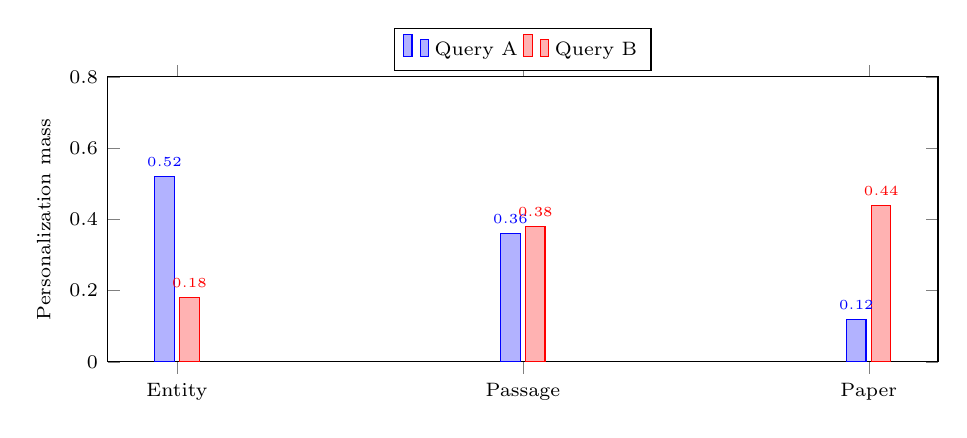
\begin{tikzpicture}
\begin{axis}[
    ybar,
    bar width=7pt,
    width=\columnwidth,
    height=5.2cm,
    ylabel={Personalization mass},
    symbolic x coords={Entity,Passage,Paper},
    xtick=data,
    ymin=0,
    ymax=0.8,
    legend style={
        at={(0.5,1.02)},
        anchor=south,
        legend columns=2,
        font=\scriptsize
    },
    tick label style={font=\scriptsize},
    label style={font=\scriptsize},
    nodes near coords,
    every node near coord/.append style={
        font=\tiny,
        /pgf/number format/.cd,
        fixed,
        precision=2
    }
]
\addplot coordinates {
    (Entity,0.52)
    (Passage,0.36)
    (Paper,0.12)
};
\addplot coordinates {
    (Entity,0.18)
    (Passage,0.38)
    (Paper,0.44)
};
\legend{Query A, Query B}
\end{axis}
\end{tikzpicture}

\caption{
Illustrative visualization of query-specific personalization mass.
The final version should replace the illustrative values with the
empirical distribution obtained from the test set.
}
\label{fig:mass}
\end{figure}


% ============================================================
% 6.5 Similarity Reweighting Baseline
% ============================================================
\subsection{Is the Gain Merely Similarity Reweighting?}

A natural alternative to the learned policy is to directly multiply
the initial personalization vector by query-node similarity:
\begin{equation}
r'_v
=
r_v
\cdot
\max(0,s(\q,v)).
\label{eq:cosine-baseline}
\end{equation}

This baseline tests whether the performance improvement can be
explained simply by favoring semantically similar nodes.

In contrast, \method learns node-type-specific thresholds, slopes,
and routing weights. Therefore, if \method substantially outperforms
the cosine baseline, the result provides evidence that the learned
policy captures retrieval behavior beyond direct semantic
reweighting.

% TODO: Add quantitative comparison.


% ============================================================
% 7. Discussion
% ============================================================
\section{Discussion}

\subsection{What Does the Policy Learn?}

The policy should not be interpreted as learning an independent model
for each query. Instead, all queries share the same policy
$\policy$, while the policy generates different control variables
conditioned on the query:
\begin{equation}
\q_1\rightarrow\Theta_{\q_1},
\qquad
\q_2\rightarrow\Theta_{\q_2}.
\end{equation}

Thus, \method can be interpreted as learning a
\emph{shared query-conditioned retrieval strategy}.

The resulting personalization vector is query-specific:
\begin{equation}
\reset_{\q_1}\neq\reset_{\q_2}.
\end{equation}

This distinction is important. The model does not train a separate
policy for every query. Instead, it learns a general mapping from
query semantics to retrieval behavior.

\subsection{Personalization Versus Graph Propagation}

The proposed method adapts the personalization mechanism rather than
the graph transition matrix. This design provides two advantages.

First, it preserves the original graph structure and therefore avoids
introducing additional graph parameters or changing the semantics of
existing edges.

Second, it provides a clean interface between learned semantic
matching and graph propagation. The policy determines where query
relevance should enter the graph, while PPR determines how that
relevance propagates through graph structure.

This separation can be summarized as:
\begin{equation}
\boxed{
\text{Policy: where to start}
\quad+\quad
\text{PPR: how to propagate}
}
\end{equation}

\subsection{Why Multi-Granularity Matters}

Entity, passage, and paper nodes encode different levels of semantic
information. Entity nodes provide fine-grained semantic anchors,
passages provide direct textual evidence, and papers provide
higher-level document context.

A fixed mixture of these node types assumes that all queries benefit
from the same balance. The learned weights $w_T(\q)$ relax this
assumption and allow the retrieval strategy to change with query
semantics.


% ============================================================
% 8. Limitations
% ============================================================
\section{Limitations}

Several limitations remain.

First, the current policy modifies the personalization vector but does
not directly modify the graph transition matrix. Therefore, the graph
structure itself remains query-independent.

Second, the policy currently uses a relatively compact parameterization
with one threshold and one slope for each node type. More expressive
node-level policies could potentially model finer-grained retrieval
preferences.

Third, the effectiveness of the method depends on the quality of the
initial fact retrieval and node embeddings because these components
provide the initial personalization signal and semantic similarity
used by the gate.

Finally, the current experiments focus on retrieval recall. Future
work should investigate whether the improved retrieval translates
into improvements in downstream question answering and generation.


% ============================================================
% 9. Conclusion
% ============================================================
\section{Conclusion}

We presented \method, a query-adaptive personalization policy for
multi-granular graph retrieval. Rather than applying the same PPR
personalization strategy to every query, \method uses a shared
query-conditioned policy to dynamically control granularity allocation,
semantic selectivity, and diffusion persistence.

The resulting node gates reweight the personalization vector before
PPR while preserving the original graph transition matrix. This
creates a clear separation between learned query-specific
personalization and graph-based propagation.

Experimental results show substantial improvements over the underlying
PPR retrieval baseline, with Recall@5 increasing from 77.05\% to
89.05\% and Recall@10 increasing from 82.15\% to 93.80\%. These
results support the central hypothesis that graph retrieval benefits
from adapting its personalization strategy to the semantic
characteristics of each query.

% ============================================================
% References
% ============================================================
\bibliographystyle{IEEEtran}
\bibliography{references}

\balance

\end{document}
